\documentclass[a4paper]{article}
%\usepackage{newtxtext}
\usepackage[T2A]{fontenc}
\usepackage[utf8]{inputenc}
\usepackage[russian]{babel}
\usepackage[lmargin=30mm,rmargin=15mm]{geometry}
\usepackage[]{graphicx}

\begin{document}
\hfill
%\parbox{23mm}{dsdsd}
\parbox{75mm}{\centerКакой-то адрес\\Вторая строка\\[3mm]Адресат А.А.}
	
\begin{figure}[t]
	\centering
	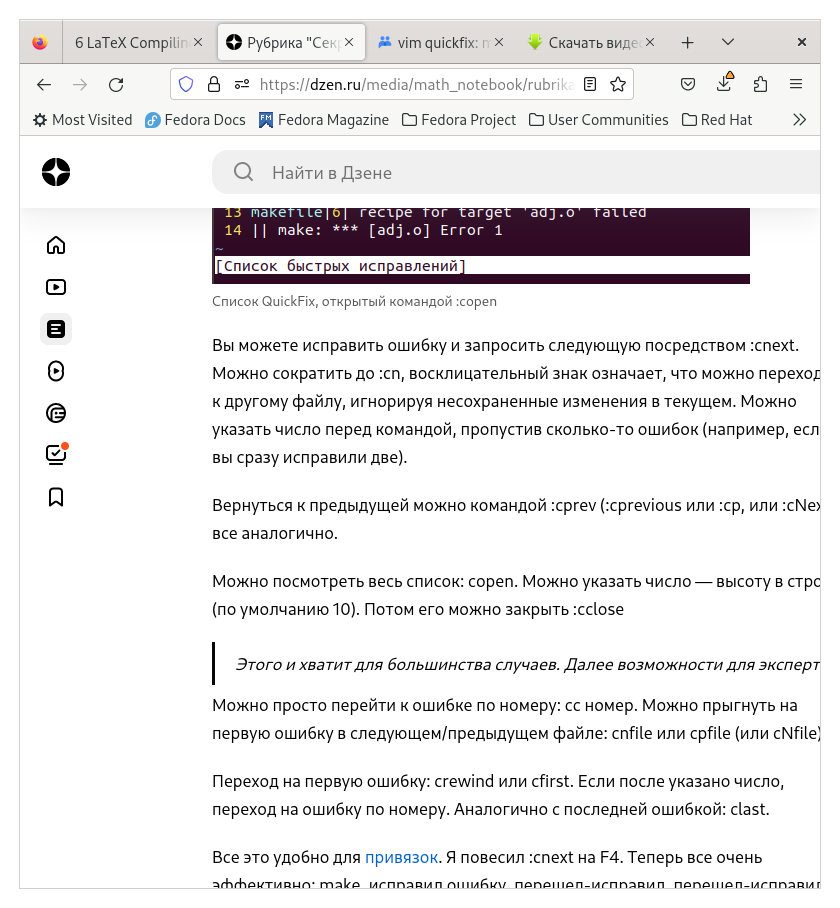
\includegraphics[width=.7\textwidth]{screenshot-firefox.png}
	\caption{Снимок экрана}
	\label{fig:screenshot}
\end{figure}

%\vskip{15mm}
Это первый абзац нового документа. Проверяем перемещение. Здесь мы просто будем опробовать различные функции 
плагина для работы \texttt{Vim} с \LaTeX.
На рисунке \ref{fig:screenshot} что-то показано. 

proba 
$$\frac{a+b}{a-b}$$
\begin{quote}
  Пример какого-то текста.
\end{quote}
\begin{equation}
   \Xi = \sqrt{2x+b} 
  \label{equation}
\end{equation}
\begin{center}
	Этот текст выровнен по центру.
\end{center}
Сейчас будет объемный абзац текста. Набран он для того, чтобы можно было проверить работу
\texttt{latexsuite} в режиме обработок ошибок компиляции. Сначала сделаем некоторую таблицу.
\begin{table}
	\centering
	\begin{tabular}{|c|l|p{3cm}|}
		\hline
		\textnumero&должность&ФИО\\
		\hline
		1.&начальник отдела&Иванов Иван Иванович\\
		2.&его заместитель&Тюльпанов Тюльпан Утюгович\\
		\hline
	\end{tabular}
	\caption{Штатное расписание}
	\label{tab:state-department}
\end{table}
После объявления таблицы продолжается абзац. Ещё несколько предложений нужно добавить в абзац.
Посмотрим, что из этого получится. Абзац должен быть достаточно большой. Добавим в него формулу, 
размещаемую внутри строки. $\sqrt{a_{12}+b^2} = a^2+b^2$.

Далее мы вставим в текст таблицу. Для полноты эксперимента код, создающий таблицу, будет размещен 
в другом файле. Файл этот назовем \texttt{second.tex}.
\begin{table}
\begin{table}
	\centering
\begin{tabular}[t]{|c|l|r|c|}
	\hline
	\textnumero&лево&право&примечание\\
	1.&Слово&Команда&Что-то еще добавлено\\
	2.&Команда&Слово&Здесь все наоборот\\
	\hline
\end{tabular}
\label{tab:from-second.tex}
\caption{способы выравнивания}
\end{table}

\label{tab:from-second.tex}
\end{table}
Таблица, описанная в файле \texttt{second.tex} показана в таблице~\ref{tab:from-second.tex}.
Пробуем автодополнение команд. Сейчас я постараюсь ввести команду. 

\end{document}
